\chapter{Related work}
\label{chap:related}

This chapter presents references to research work in domain of modelling processes
governing evolution of karst aquifers along with small summaries. This
description will be helpful in explaining design decisions made in programming
project, especially in area of input data formats.

Some visualisation techniques used previously for caved terrains in various
contexts will also be presented.

\section{Modelling karst aquifers}

As karst aquifers contain network of fractures (see \autoref{chap:karstification})
a simulation of flow and chemical reactions in single fracture is the basic
building block of presented models.

These fractures are connected to form larger, two or three--dimensional networks,
that represent whole conduits.

First attempts to describe processes taking place during evolution of karst
aquifers with numerical models took place in early 1980's \parencite[p. 3]{hiller2013}.
\Cite{Buhmann1985189} developed numerical model for ternary chemical system
(\cee{CaCO3}--\cee{CO2}--\cee{H2O}) in open systems (where \cee{CO2} is exchanged
with atmosphere) and for closed ones \parencite{Buhmann1985109}.

\subsection{Single fracture simulation}

With these dissolution models in place, several models of single conduit simulation
were presented \parencite[p. 4]{hiller2013}.

Single fracture is modelled as a circular conduit in the intersection
of fissure and bedding plane \parencite{Kaufmann200962} or as a space between
two parallel walls of rock separated by aperture of some width \parencite{dreybrodt2002}.

\subsection{Two--dimensional simulations}

Single conduit one--dimensional models were later expanded into second dimension
by combining set of conduits into a connected network \parencite[pp. 4--5]{hiller2013}.
In such networks, fractures are organized into uniform, regular structure.

\subsection{Three--dimensional simulations}

With more powerful computational resources, researchers started to look into
three--dimensional models that could finally provide insight into evolution
of real--life karst aquifers. Such models were proposed by
\cites{annable2003}{WRCR:WRCR9525}{Kaufmann2010241}.

Work by \cite{hiller2013} summarizes current state of three--dimensional models.
His thesis contains overview of modelling techniques and approaches. Simulation
of real--live karst aquifer near dam--site is presented that matches
observations. This shows validity of proposed models.

These three--dimensional models also store data as a uniform grid of fractures.
This fact heavily infulenced the design of data structures used throughout
programming part of this thesis described in \autoref{chap:project}.

\section{Visualisation techniques}

Rendering techniques that touched the issue of cave rendering never tried to
provide both physical accuracy and visually appealing graphics.

In \cite{gpugems3ch01} a method for rendering procedural terrains is described
that in some circumstances can generate caved structures. Similar to programming
project of this thesis, presented method uses Marching Cubes algorithm
(see \autoref{chap:marchingcubes}) implemented on GPU\footnote{Albeit in shaders,
not with any GPGPU solution}. Volume data is generated through carefully crafted
density functions based on noise sampling and various scalar
functions that are easily computable in shaders.

\Cite{forstmann2005} proposed method of on--the--fly rendering of procedural
terrains that may also contain caves. It uses hierarchy of nested clip--boxes
for LOD\footnote{Level of detail} calculation to reduce workload of the GPU.

\Cite{hiller2013} developed \emph{KARSTTOOL} -- a MATLAB application that
is capable of plotting various parameters of three--dimensional fracture net
computed by running karst evolution simulation with \emph{KARSTAQUIFER}
simulator introduced in \cite{Kaufmann200962}. This program doesn't strive to provide visually rich renders; it's
aimed at researchers that want to visualise various parameters of simulated
karst aquifer like \cee{CO2} or \cee{HCO3} concentration. Screenshot of KARSTOOL
application is presented below.

\begin{figure}[h]
  \begin{center}
    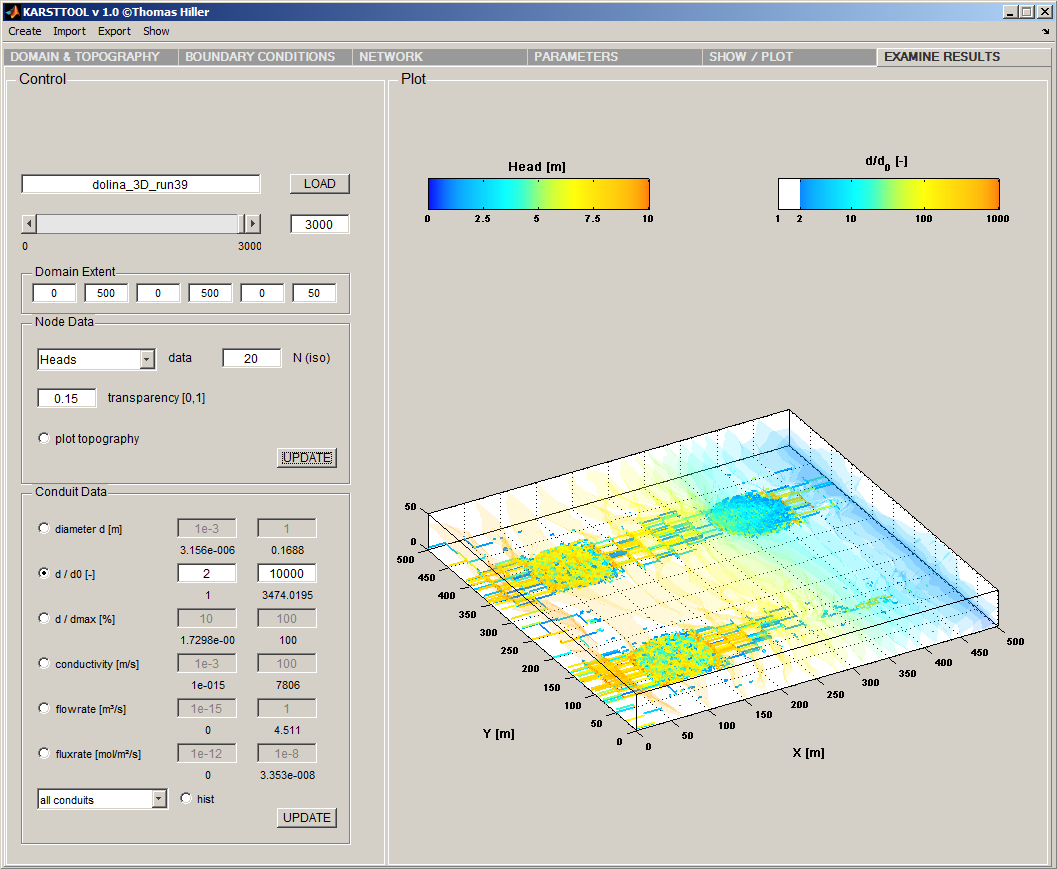
\includegraphics[width=\textwidth]{chapters/relatedwork/karsttool.png}
  \end{center}
  \caption{Screenshot of KARSTTOOL application. Results tab is shown that
  presents visualisation of simulation.}
  \label{fig:karsttool}
\end{figure}

\subsection{Surveying software}

Research around cave rendering is also done for cave surveying software.
These specialized programs allow speleologists to capture data about structure
of caves by manual or device--assisted measurement during exploration and plot
the gathered data. Examples of open--source programs of this kind are
\emph{Therion}\footnote{\url{http://therion.speleo.sk/index.php}} and
\emph{Survex}\footnote{\url{http://www.survex.com}}. More comprehensive list,
albeit outdated, is available at British Cave Research Association Cave Surveying
Special Group (\url{http://csg.bcra.org.uk/software.html}). Screenshot of 3D
plot of graphic survey data from Therion is presented below.
\begin{figure}[h]
  \begin{center}
    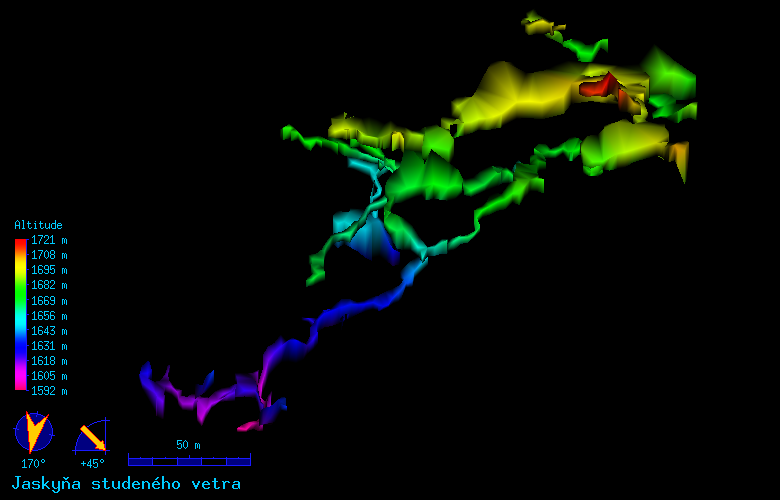
\includegraphics[width=\textwidth]{chapters/relatedwork/therion.png}
  \end{center}
  \caption{3D visualisation of cave survey data from Therion application}
  \label{fig:therion}
\end{figure}
